\documentclass[a4paper]{article}
\usepackage[colorlinks=true,allcolors=blue]{hyperref}
\usepackage{amsmath}
\usepackage{graphicx}
\usepackage{amsfonts}
\usepackage[none]{hyphenat} %this is not necessary for the students to figure out, but a good thing to know
% it also sometimes gets rid of the overfull/underfull box warning



\title{Exercise 2}
\author{Me, myself and I}
\date{\today}

\begin{document}


\maketitle
	
\section*{Tables}

\noindent Let's first try our hand at a table containing some notable novels. The information on the country and year of publication comes from \href{https://en.wikipedia.org/wiki/Main_Page}{Wikipedia}.\footnote{Use the \textit{hyperref} package to add links to your document and add \texttt{[colorlinks=true,allcolors=blue]} before the package name to make all links and references blue.}

\begin{center}
\begin{tabular}{||l | l | l | l ||} 
 \hline
 Title & Author & Country & Year\\ [1ex] 
 \hline\hline 
 The Tale of Genji & Murasaki Shikibu & Japan & Before 1021 \\  
 \hline
 Journey to the West & Wu Cheng'en & Ming China & c. 1592 \\
 \hline
 Pride \& Prejudice & Jane Austen & England & 1813 \\ 
 \hline
 War \& Peace & Leo Tolstoy & Russia & 1865-67 \\
 \hline
  The Great Gatsby & F. Scott Fitzgerald & United States & 1925 \\
 \hline
\end{tabular}
\end{center}

\section*{Formulas and mathematical notation}
\begin{equation*}
    E = mc^2
\end{equation*}


\begin{align*} 
2x - 6 &=  8 \\ 
2x &=  8 + 6\\
  x  &= \frac{8 + 6}{2}\\
  x &= 7
\end{align*}

\begin{center}
\noindent N\textsubscript{2} + 3H\textsubscript{2} $\rightarrow$ 2NH\textsubscript{2}    
\end{center}


\begin{equation} \label{eq:resistance}
    R = \frac{L}{{\sigma A}} = \frac{{\rho L}}{A}
\end{equation}	

\noindent Equation \ref{eq:resistance} describes electrical resistance. The symbol $\sigma$ is called sigma, $\rho$ is called rho.\\

\noindent $\mathbb{N}$ denotes the set of natural numbers. Therefore, $ \mathbb{N}=\{1,2,3,\ldots,\infty\} $

\newpage

\section*{Images}

Go to \href{https://commons.wikimedia.org/wiki/Category:Featured_pictures_of_Ukraine#/media/File:21-224-5054_NNP_Synevyr_RB_18.jpg}{this link} on Wikimedia Commons and download the picture (to save space, don't download the original file, but the preview). Then insert it here, as shown below.
\begin{figure}[h!]
    \centering
    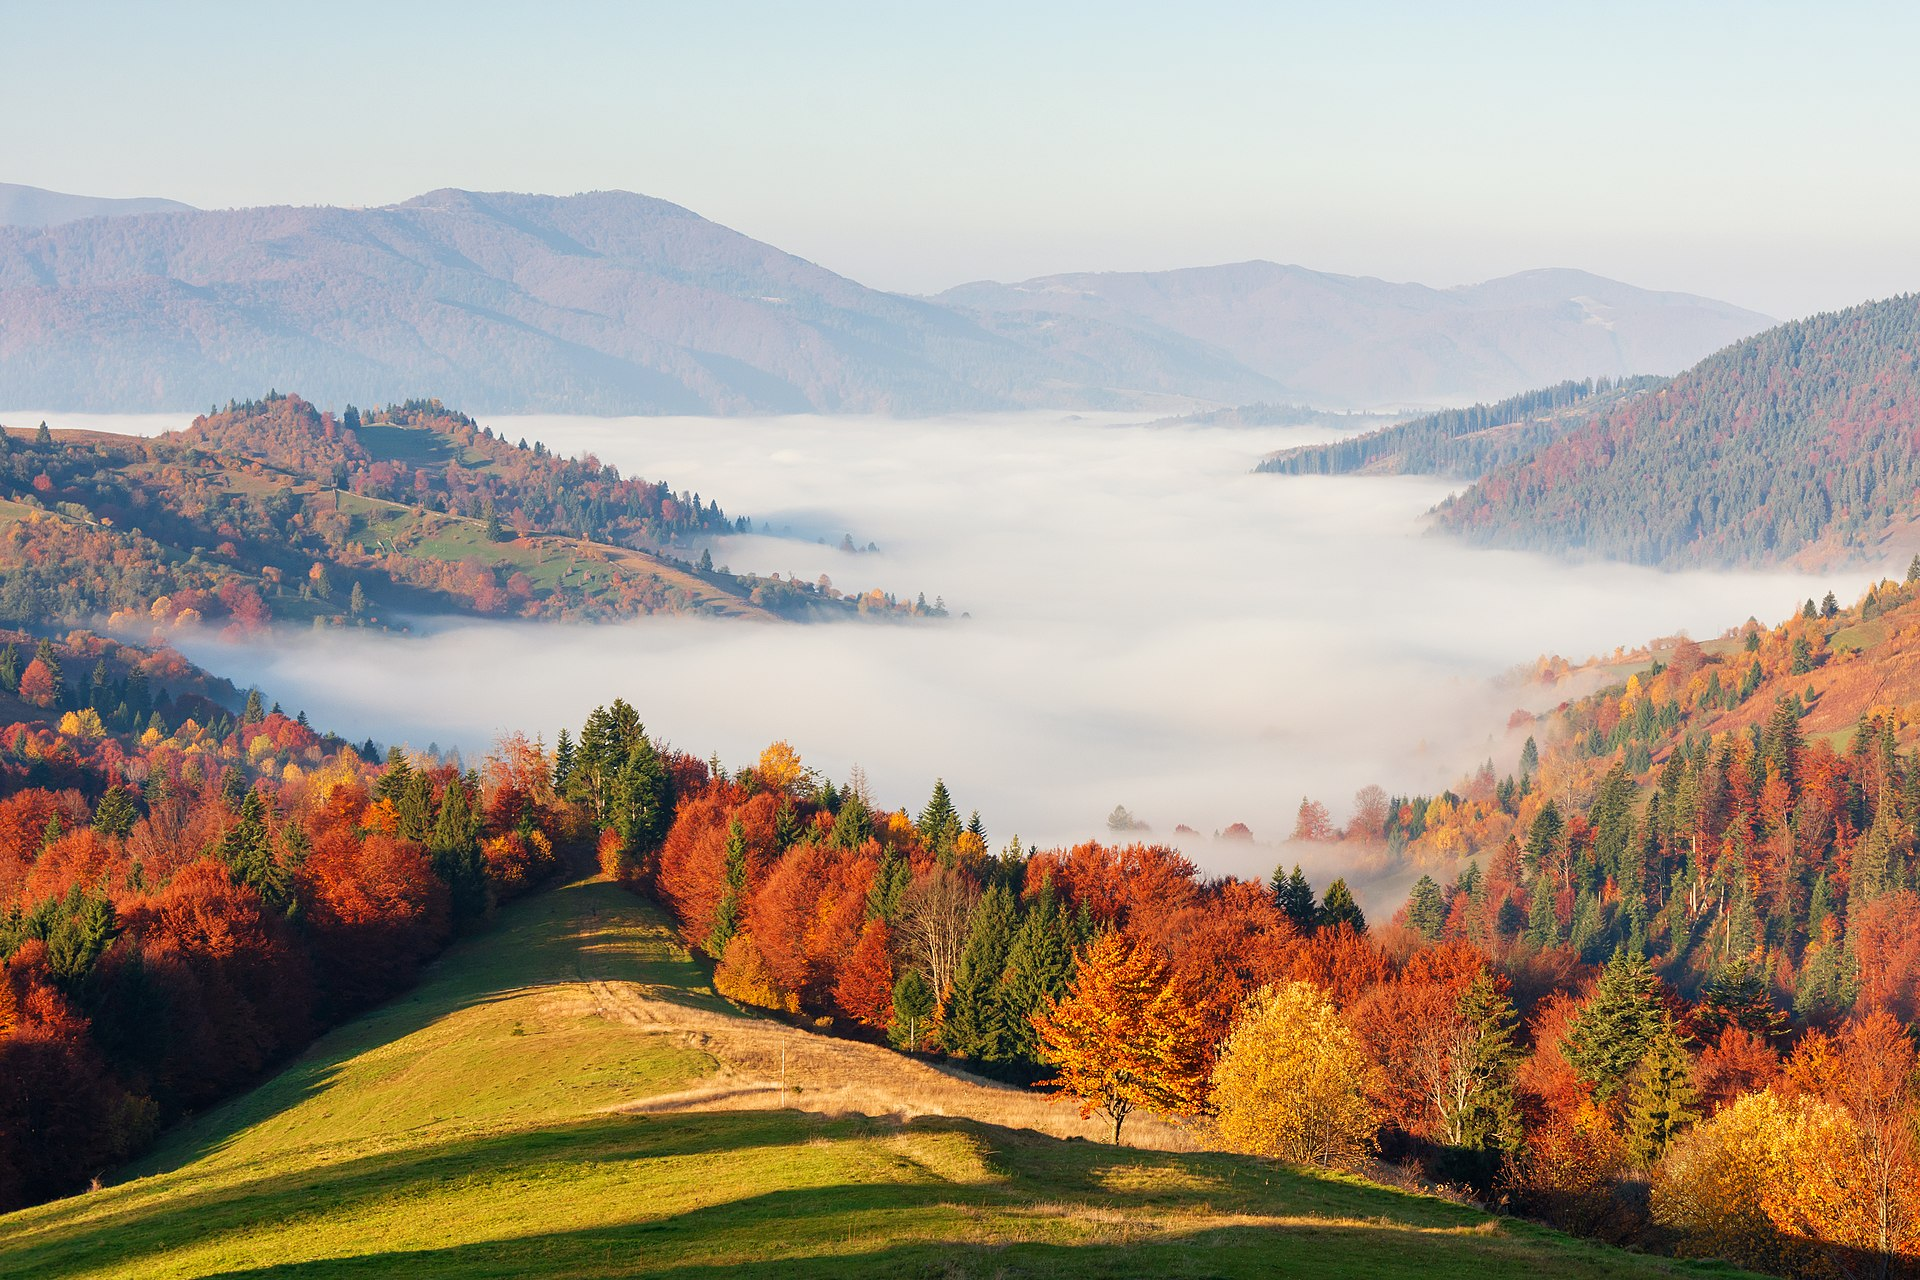
\includegraphics[width=\textwidth]{ukraine_wikimedia.jpg}
    \caption{Source: \href{https://commons.wikimedia.org/wiki/File:21-224-5054_NNP_Synevyr_RB_18.jpg}{Wikimedia Commons}}
    \label{fig:ukraine_wikimedia}
\end{figure}

Figure \ref{fig:ukraine_wikimedia} shows the National Nature Park Synevyr in Ukraine.

\newpage

Now scale it down to 5\% of its size (mind the placement!) and reference it like so: figure \ref{fig:ukraine_wikimedia_scaled} shows the same picture as before, but scaled to 5\% of its size.

\begin{figure}[b!]
    \centering
    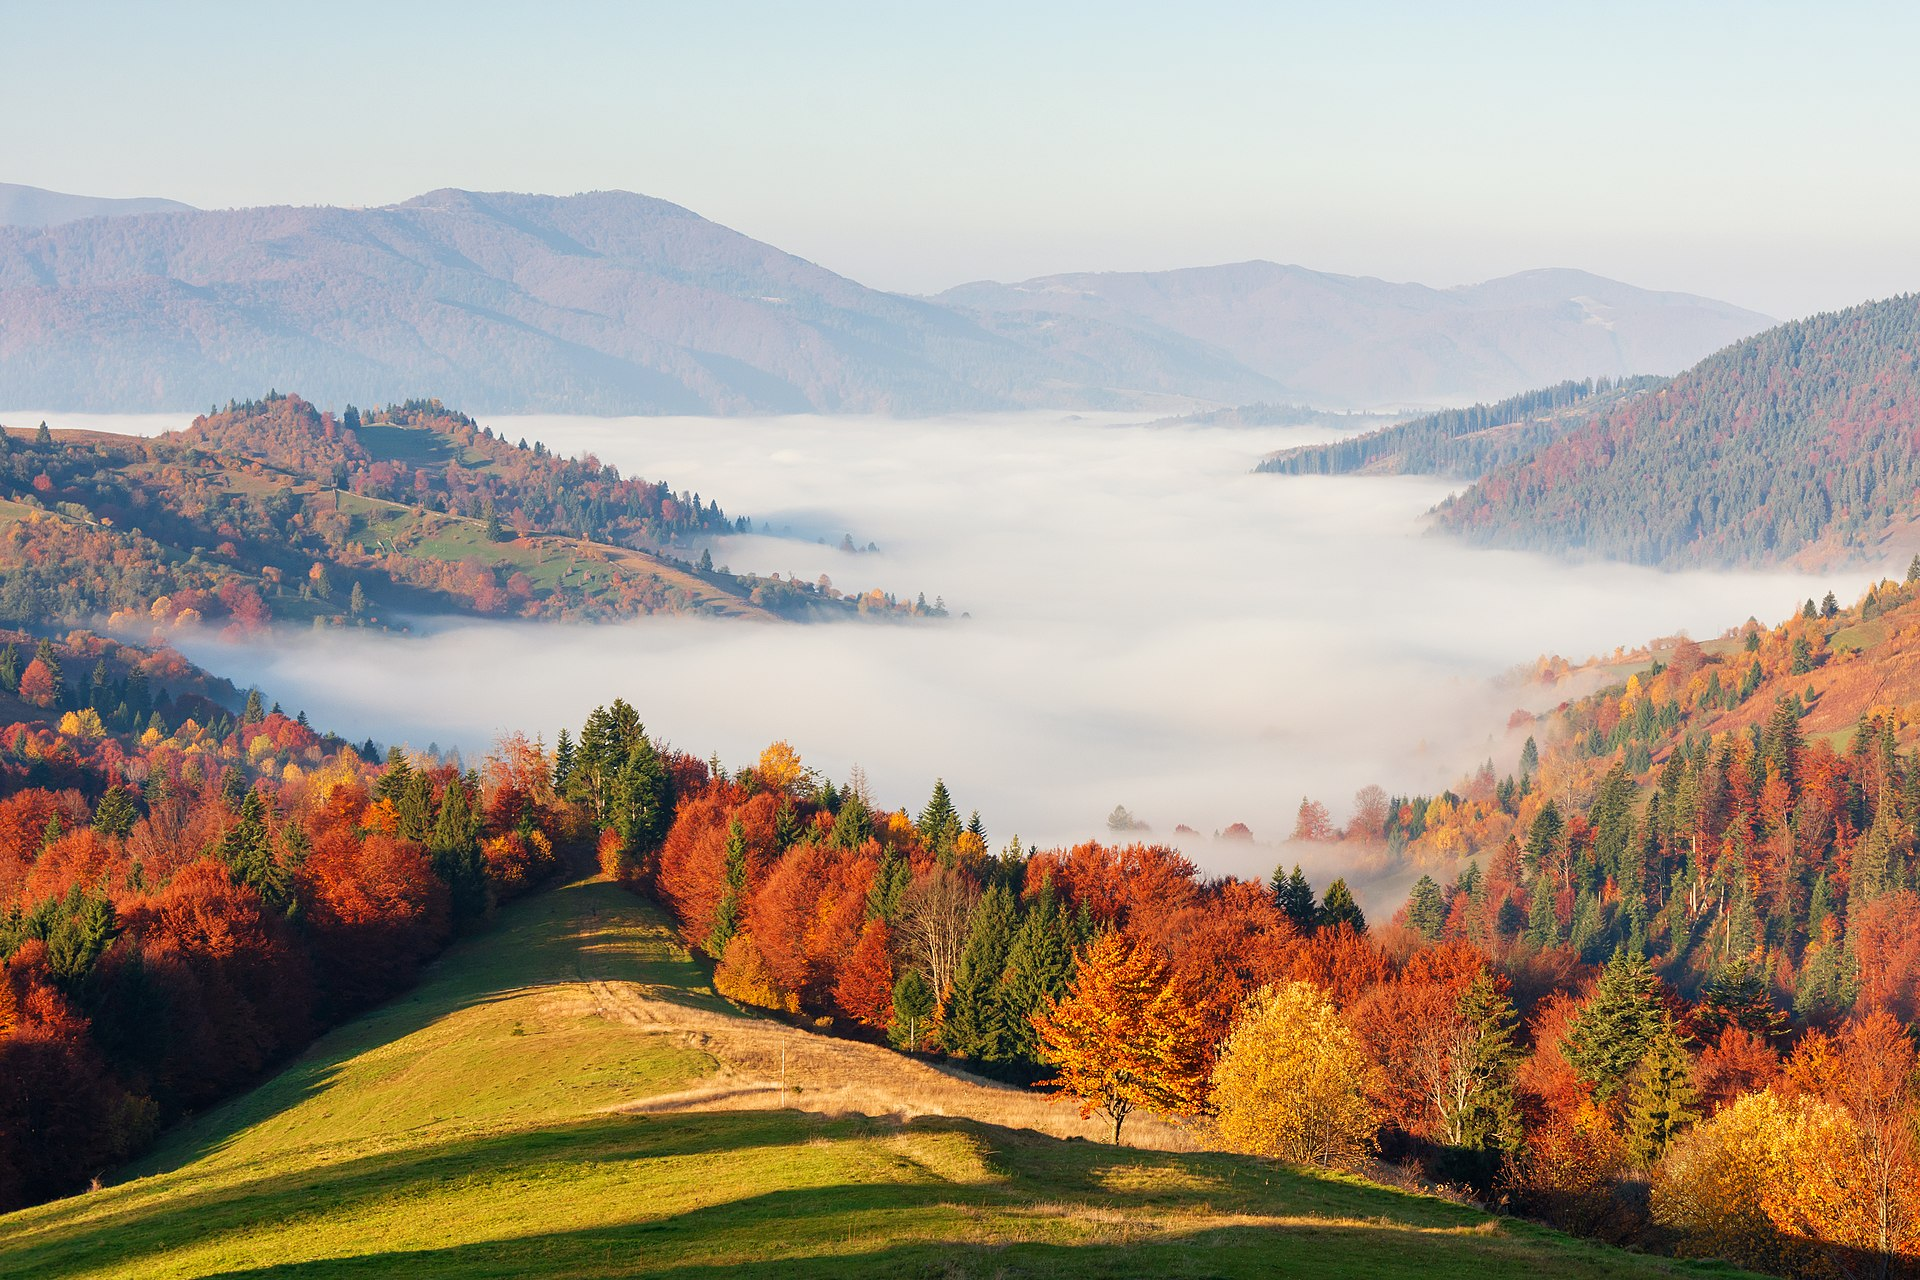
\includegraphics[scale=0.05]{ukraine_wikimedia.jpg}
    \caption{Scaling it down}
    \label{fig:ukraine_wikimedia_scaled}
\end{figure}

		
\end{document}